\section{Двоичное дерево поиска}



Пусть мы хотим завести некоторую структуру данных, в которой можно хранить элементы типа $T$ с компаратором $cmp$ и поддержкой таких операций, как $insert(x)$, $erase(x)$, $exists(x)$ (как, например, в set). Такое можно сделать через хэш-таблицы или через vector за $O(n)$ на операцию, но мы сделаем по-другому. 
Давайте сделаем двоичное дерево, где в каждой вершине будет написано какое-то из добавленных значений, и где для каждого поддерева будет выполнено следующее условие: значения всех элементов из левого поддерева меньше, чем в корне, а из правого больше. \\ 

\begin{center} 
    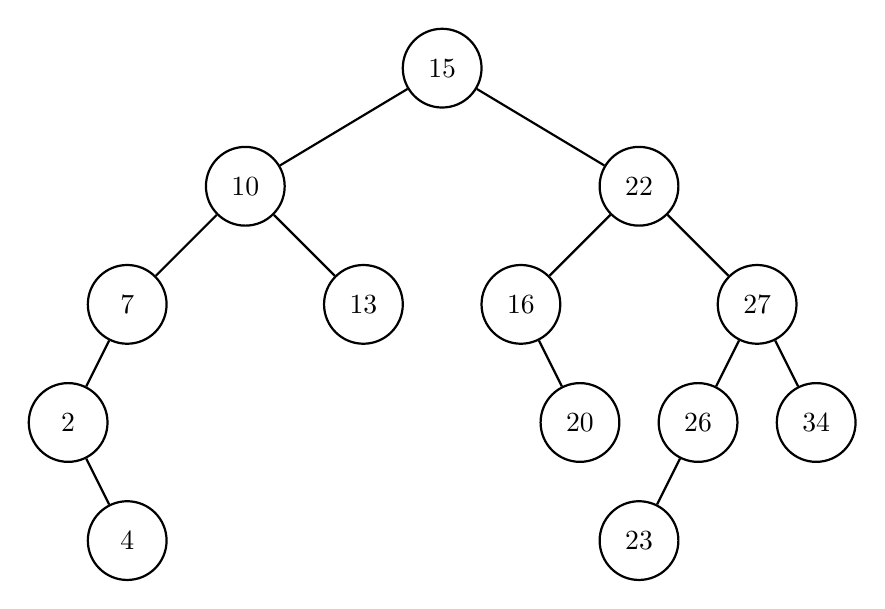
\begin{tikzpicture}[
            thick,
            every node/.style = {draw, circle, minimum size=10mm},
            level 1/.style = {sibling distance=50mm},
            level 2/.style = {sibling distance=30mm}, 
            level 3/.style = {sibling distance=15mm}, 
            level distance = 15mm
        ]
        \node {15}
            child {node {10}
                child {node {7}
                    child {node {2}
                        child[missing]
                        child {node {4}}
                    }
                    child[missing]
                }
                child {node {13}}
            }
            child {node {22}
                child {node {16}
                    child[missing]
                    child {node {20}}
                }
                child {node {27}
                    child {node {26}
                        child {node {23}}
                        child[missing]
                    }
                    child {node {34}}
                }
            };
    \end{tikzpicture}
\end{center}

В идеале, ДДП -- это ``протокол'' бинарного поиска в массиве. То есть в корне поддерева лежит центральный элемент соответствующего подотрезка массива, в левом поддереве тоже самое, при условии, что элемент в корне оказался больше, чем нужный, а справа, если меньше. \\

\begin{center} 
    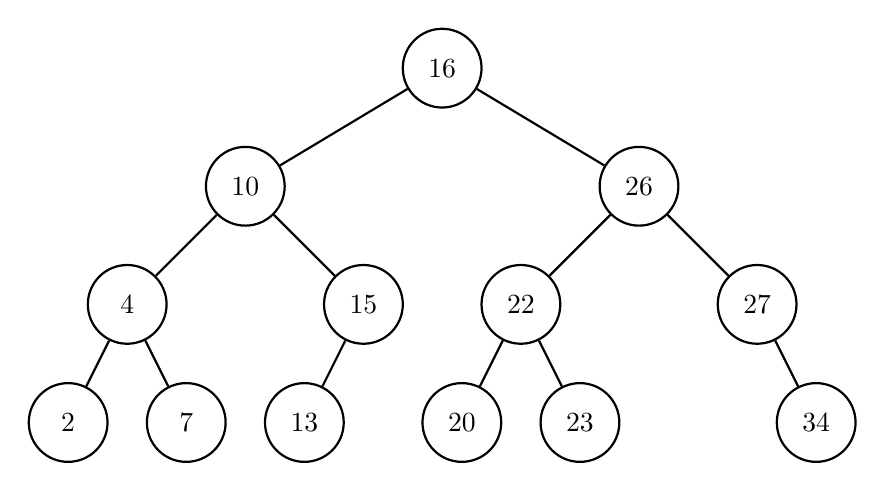
\begin{tikzpicture}[
            thick,
            every node/.style = {draw, circle, minimum size=10mm},
            level 1/.style = {sibling distance=50mm},
            level 2/.style = {sibling distance=30mm}, 
            level 3/.style = {sibling distance=15mm}, 
            level distance = 15mm
        ]
        \node {16}
            child {node {10}
                child {node {4}
                    child {node {2}}
                    child {node {7}}
                }
                child {node {15}
                    child {node {13}}
                    child[missing]
                }
            }
            child {node {26}
                child {node {22}
                    child {node {20}}
                    child {node {23}}
                }
                child {node {27}
                    child[missing]
                    child {node {34}}
                }
            };
    \end{tikzpicture}
\end{center}

\begin{problem}
    Сколько существует различных ДДП, в которых лежат все целые числа от 1 до $n$? 
\end{problem}

\begin{solution}
    Рассмотрим следующее отображение из множества всех ДДП размера $n$ в множество всех ПСП длины $2n$: на месте корневого элемента поставим закрывающую скобку, левее левого поддерева поставим открывающую скобку, и проделаем так рекурсивно в обоих поддеревьях. Рассмотрим другое отображение в обратную сторону: посмотрим на первую скобку и найдем соответствующую ей закрывающую, внутри этих скобок и правее них есть какие-то ПСП (возможно, пустые). На месте закрывающей скобки поставим корень, слева подвесим то, что получилось во внутренней ПСП, справа то, что в правой ПСП. Теперь докажем, что эти два отображения обратны друг другу. Пусть мы по какому-то дереву получили ПСП, давайте заметим, что во внутренней ПСП (из которой мы получим новое левое поддерево) столько же пар скобок, сколько было и будет в левом поддереве. Из этого факта легко по индукции доказать, что из левой ПСП (как и из правой) можно сделать только одно ДДП, которое совпадает с тем, из которого мы получили это ПСП. Таким образом, мы доказали, что такое отображение - это биекция между множеством ПСП и ДДП, тогда количество ДДП размера $n$ -- это $n$-тое число Каталана.
\end{solution}

\begin{example}
    Одна вершина -- (). Вершина, у которой два ребенка -- (())(). Бамбук из 5 вершин, где каждый ребенок правый -- ()()()()(), а если каждый ребенок левый -- ((((())))).
    Двум ДДП, которые изображены выше, соответствуют следующие ПСП: (((()()))())(()())((()))(), (((())())(()))((())())()().
\end{example}



\subsection{Обходы дерева}



В коде у нас будет отдельный объект для вершины дерева.
\begin{lstlisting}
    struct Node {
        TKey key;
        Node *left, *right;
    }
\end{lstlisting}

Существует всего 3 обхода дерева. 

\begin{enumerate}
    \item Обход по принципу "сначала я, потом дети":
    \begin{lstlisting}
    void preOrder(Node* node) {
        if (!node) {
            return;
        }
        print(node->key);
        preOrder(node->left);
        preOrder(node->right);
    }
    \end{lstlisting}
    \item Обход по принципу "сначала дети, потом я":
    \begin{lstlisting}
    void postOrder(Node* node) {
        if (!node) {
            return;
        }
        postOrder(node->left);
        postOrder(node->right);
        print(node->key);
    }
    \end{lstlisting}
    $Pre$- и $PostOrder$ могут быть использованы в любых деревьях, не только в ДДП. Еще можно заметить, что в таком выводе поддерево будет являться каким-то подотрезком выходного массива.
    \item "Эксклюзивный" обход, который можно использовать только в ДДП, по принципу "ни туда, ни сюда":
    \begin{lstlisting}
    void inOrder(Node* node) {
        if (!node) {
            return;
        }
        inOrder(node->left);
        print(node->key);
        inOrder(node->right);
    }
    \end{lstlisting}
\end{enumerate}

Польза $inOrder$ обхода заключается в том, что в нем элементы записаны в таком же порядке, как они идут в реальном дереве слева направо, поэтому это часто бывает полезно для дебага.

\begin{example}
    Для данного дерева выводы обходов будут следующими: \\
    \begin{figure}[htbp]
        \begin{center} 
            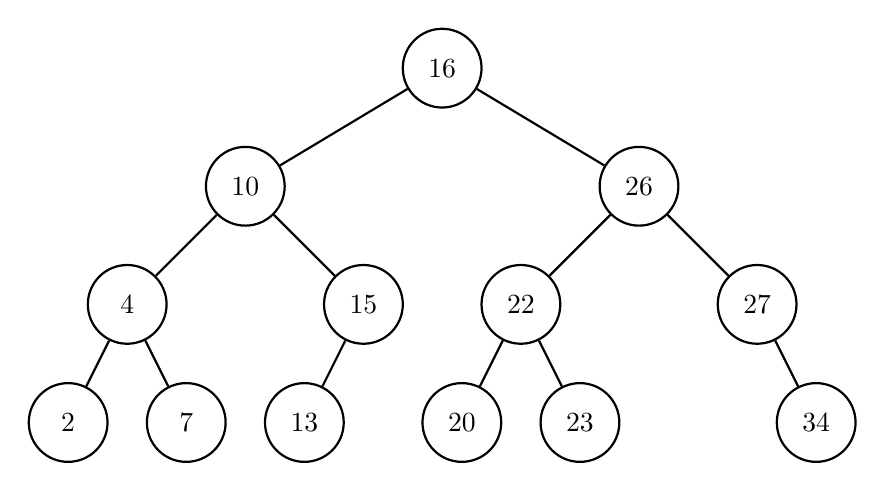
\begin{tikzpicture}[
                    thick,
                    every node/.style = {draw, circle, minimum size=10mm},
                    level 1/.style = {sibling distance=50mm},
                    level 2/.style = {sibling distance=30mm}, 
                    level 3/.style = {sibling distance=15mm}, 
                    level distance = 15mm
                ]
                \node {16}
                    child {node {10}
                        child {node {4}
                            child {node {2}}
                            child {node {7}}
                        }
                        child {node {15}
                            child {node {13}}
                            child[missing]
                        }
                    }
                    child {node {26}
                        child {node {22}
                            child {node {20}}
                            child {node {23}}
                        }
                        child {node {27}
                            child[missing]
                            child {node {34}}
                        }
                    };
            \end{tikzpicture}
        \end{center}
    \end{figure}
    \begin{enumerate}
        \item $PreOrder$: 16, 10, 4, 2, 7, 15, 13, 26, 22, 20, 23, 27, 34
        \item $PostOrder$: 2, 7, 4, 13, 15, 10, 20, 23, 22, 34, 27, 26, 16
        \item $InOrder$: 2, 4, 7, 10, 13, 15, 16, 20, 22, 23, 26, 27, 34
    \end{enumerate}
    Обратите внимание, что в выводе $InOrder$ обхода ДДП всегда будет отсортированный массив.
\end{example}



\subsection{Операции в двоичном дереве поиска}



\begin{enumerate}
    \item $exists(x)$ \\
    Посмотрим на корень, если это $x$ - то мы его нашли. Если же он меньше, чем $x$, то продолжим поиск в правом поддереве, если больше - то в левом. Если в итоге пришли в пустую вершинку (то есть хотим перейти в пустое поддерево), то данного элемента нет в ДДП. Такая проверка работает за $O(h)$, где $h$ - высота дерева.
    \item $insert(x)$ \\
    Немного модифицируем $exists(x)$ - если мы нашли его в дереве, то никак не будем менять наше дерево, а если нет, то в том месте, где мы попытались перейти в пустое поддерево, вместо этого пустого поддерева подвесим тот элемент, который мы хотим. Этот алгоритм тоже работает за $O(h)$.
    \item $erase(x)$ \\
    Для начала проверим, есть ли данный элемент в дереве, и если есть, то дойдем до него и рассмотрим 3 случая:
    \begin{enumerate}
        \item У $x$ нет детей, тогда просто удалим его.
        \item У $x$ есть 1 ребенок, тогда просто удалим его, а на его место поставим этого самого ребенка.
        \item У $x$ есть 2 ребенка, тогда заметим, что если мы возьмем самый левый элемент из правого поддерева, то мы получим наименьший элемент, который больше, чем $x$, причем у которого нет левого ребенка. Меняем местами его и $x$, и можем спокойно удалить $x$, т. к. теперь у него не более, чем 1 ребенок. \\
        \begin{figure}[htbp]
            \begin{tabular}{m{6cm}m{6cm}m{6cm}}
                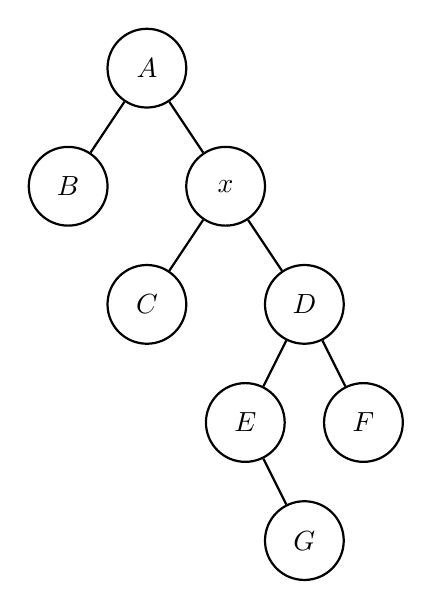
\begin{tikzpicture}[
                        thick,
                        every node/.style = {draw, circle, minimum size=10mm},
                        level 1/.style = {sibling distance=20mm},
                        level 2/.style = {sibling distance=20mm}, 
                        level 3/.style = {sibling distance=15mm}, 
                        level distance = 15mm
                    ]
                    \node {$A$}
                        child {node {$B$}}
                        child {node {$x$}
                            child {node {$C$}}
                            child {node {$D$}
                                child {node {$E$}
                                    child[missing]
                                    child {node {$G$}}
                                }
                                child {node {$F$}}
                            }
                        };
                \end{tikzpicture}
            &
                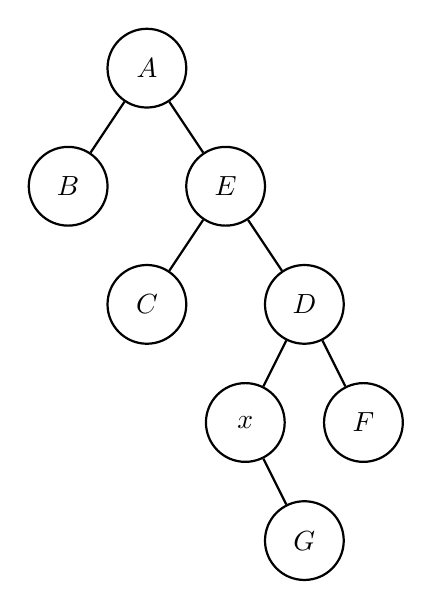
\begin{tikzpicture}[
                        thick,
                        every node/.style = {draw, circle, minimum size=10mm},
                        level 1/.style = {sibling distance=20mm},
                        level 2/.style = {sibling distance=20mm}, 
                        level 3/.style = {sibling distance=15mm}, 
                        level distance = 15mm
                    ]
                    \node {$A$}
                        child {node {$B$}}
                        child {node {$E$}
                            child {node {$C$}}
                            child {node {$D$}
                                child {node {$x$}
                                    child[missing]
                                    child {node {$G$}}
                                }
                                child {node {$F$}}
                            }
                        };
                \end{tikzpicture}
            &
                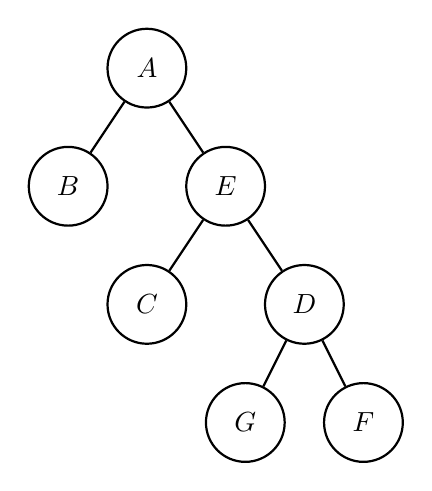
\begin{tikzpicture}[
                        thick,
                        every node/.style = {draw, circle, minimum size=10mm},
                        level 1/.style = {sibling distance=20mm},
                        level 2/.style = {sibling distance=20mm}, 
                        level 3/.style = {sibling distance=15mm}, 
                        level distance = 15mm
                    ]
                    \node {$A$}
                        child {node {$B$}}
                        child {node {$E$}
                            child {node {$C$}}
                            child {node {$D$}
                                child {node {$G$}}
                                child {node {$F$}}
                            }
                        };
                \end{tikzpicture}
            \end{tabular}
            \caption*{Третий случай, который перешел во второй, и далее удаление $x$}
        \end{figure}
    \end{enumerate}
    Таким образом мы умеем удалять за $O(h)$.
    \item $get\_max(subtree)$ \\ 
    Просто будем идти вправо до конца, получим максимум за $O(h)$.
    \item $get\_min(subtree)$ \\ 
    Аналогично максимуму, только идти будем влево.
    \item $upper\_bound(x)$ \\
    Найдем минимум в правом поддереве. Если правого поддерева нет, то будем идти обратно наверх, пока мы не пройдем вверх из левого ребенка, тогда это будет ответом. Если же мы всегда будем идти вверх из правого ребенка и дойдем так до корня, то мы вообще были максимумом всего дерева. Асимптотика: $O(h)$.
    \begin{note}
    Обычно в коде это будет сделано так: если корень не превосходит x, то ответ берем из правого поддерева, а если превосходит, то ответ либо сам корень, либо что-то из левого поддерева. Запомним значение в корне и будем идти влево, поддерживая минимальный ответ.
    \end{note}
    Полезное свойство такой реализации $upper\_bound(x)$ в том, что оно никак не меняет дерево (по модулю отложенных операций), и неасимптотически гораздо быстрее, чем, например, выражение через $split$ и $merge$. А еще, если передавать $x$ не по значению, а по указателю, то можно найти ответ даже без сравнений (таким образом можно делать, к примеру, $iterator$++).
\end{enumerate}
У всего этого есть огромный недостаток. С текущей реализацией $insert(x)$ можно сделать бамбук (если, например, вставлять элементы только по возрастанию или убыванию), тогда высота дерева будет $n$ и все операции будут работать за $O(n)$. Естественно, это очень плохо, поэтому обычно всегда используют какие-нибудь другие виды ДДП.



\section{AVL-дерево}



АВЛ - это аббревиатура, образованная первыми буквами фамилий его создателей из СССР: Адельсон-Вельский Георгий Максимович и Ландис Евгений Михайлович. Исторически, это первое когда-либо созданное сбалансированное двоичное дерево поиска, первое упоминание в статьях было в 1962 году. \\
Заметим, что всегда $h \geq log_2(n)$, и на запрос поиска ответом может быть любая из $n$ вершинок, поэтому невозможно искать элемент быстрее, чем за $O(log_2(n))$ (идея доказательства такая же, как в доказательстве худшего случая произвольной сортировки сравнениями). В этом алгоритме мы хотим так ``балансировать'' дерево, чтобы всегда было верно $h = O(log_2(n))$, таким образом, все операции, которые работают за $O(h)$, будут работать за $O(log_2(n))$.

\begin{invariant}
    У любой вершины разность высот ее детей не превышает 1.
\end{invariant}


\begin{corollary}
    Высота дерева $h$ всегда примерно равна $log_2(n)$.
\end{corollary}

\begin{proof}
    Введем функцию $minSz(h)$ со следующими ограничениями:
    $\forall h \geq 2: minSz(h) \geq minSz(h - 1) + minSz(h - 2) + 1$, $minSz(1) = 1$, $minSz(0) = 0$.
    \begin{enumerate}
        \item[Способ 1.] $\forall h \geq 2: minSz(h) \geq minSz(h - 1) + minSz(h - 2)$, тогда заметим, что $minSz(h)$ не меньше, чем $h$-тое число фибоначчи, тогда $minSz(h) = \Omega(\phi^h)$. Если размер ДДП равен $n$, то $n \geq C \phi^h \implies log_\phi(n) \geq C h$ для некоторой константы $C$, тогда $h = O(log_\phi(n)) = O(log_2(n))$.
        \item[Способ 2.] Заметим, что $minSz(h) \geq 2minSz(h - 2) + 1$. Увеличивая высоту на 2, размер дерева увеличивается примерно в 2 раза, из этого легко вывести требуемое.
    \end{enumerate}
\end{proof}



\subsection{Операции в AVL-дереве}



\begin{definition}
    Малый правый поворот -- операция на дереве, при которой происходит следующее: если был корень $X$, его левый ребенок $Y$, то после операции корнем станет $Y$, а его правым ребенком $X$, все дети $X$ и $Y$ сохранятся, кроме правого ребенка $Y$ -- он станет левым ребенком $X$. \\
    \begin{center}
        \begin{tabular}{m{6cm}m{6cm}}
            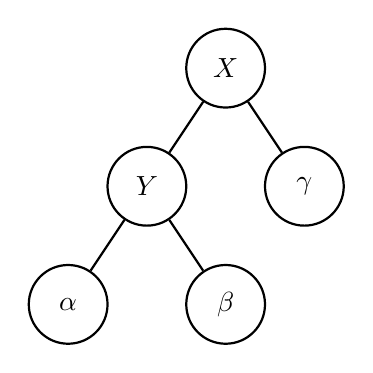
\begin{tikzpicture}[
                    thick,
                    every node/.style = {draw, circle, minimum size=10mm},
                    level 1/.style = {sibling distance=20mm},
                    level 2/.style = {sibling distance=20mm}, 
                    level 3/.style = {sibling distance=15mm}, 
                    level distance = 15mm
                ]
                \node {$X$}
                    child {node {$Y$}
                        child {node {$\alpha$}}
                        child {node {$\beta$}}
                    }
                    child {node {$\gamma$}};
            \end{tikzpicture}
        &
            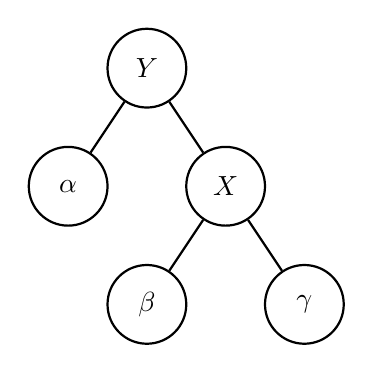
\begin{tikzpicture}[
                    thick,
                    every node/.style = {draw, circle, minimum size=10mm},
                    level 1/.style = {sibling distance=20mm},
                    level 2/.style = {sibling distance=20mm}, 
                    level 3/.style = {sibling distance=15mm}, 
                    level distance = 15mm
                ]
                \node {$Y$}
                    child {node {$\alpha$}}
                    child {node {$X$}
                        child{node {$\beta$}}
                        child{node {$\gamma$}}
                    };
            \end{tikzpicture}
        \end{tabular}
    \end{center}
\end{definition}
\begin{note}
    Аналогично определяется малый левый поворот.
\end{note}
Нетрудно доказать простой проверкой, что инвариант ДДП сохранится.

\begin{note}
    По фиксированному ребру можно сделать только один из поворотов, поэтому далее будем говорить просто ``малый поворот по ребру''
\end{note}

\begin{definition}
    Большой правый поворот -- операция на дереве, которая делает следующее: если был корень $X$, $Y$ -- левый сын $X$, $Z$ -- правый сын $Y$, то после большого правого поворота $Z$ будет корнем, его правым ребенком будет $X$, а левым -- $Y$. Все дети $X$, $Y$ и $Z$ сохранятся, кроме детей $Z$ -- правый станет левым ребенком $X$, а левый -- правым ребенком $Y$. Иначе говоря, это тоже самое, что сделать малый поворот по ребру $YZ$, а потом по ребру $XZ$. \\
    \begin{center}
        \begin{tabular}{m{6cm}m{6cm}}
            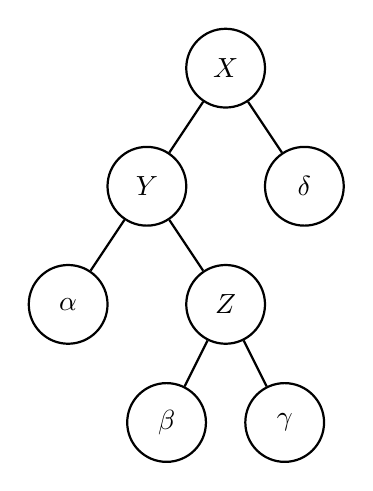
\begin{tikzpicture}[
                    thick,
                    every node/.style = {draw, circle, minimum size=10mm},
                    level 1/.style = {sibling distance=20mm},
                    level 2/.style = {sibling distance=20mm}, 
                    level 3/.style = {sibling distance=15mm}, 
                    level distance = 15mm
                ]
                \node {$X$}
                    child {node {$Y$}
                        child {node {$\alpha$}}
                        child {node {$Z$}
                            child {node {$\beta$}}
                            child {node {$\gamma$}}
                        }
                    }
                    child {node {$\delta$}};
            \end{tikzpicture}
        &
            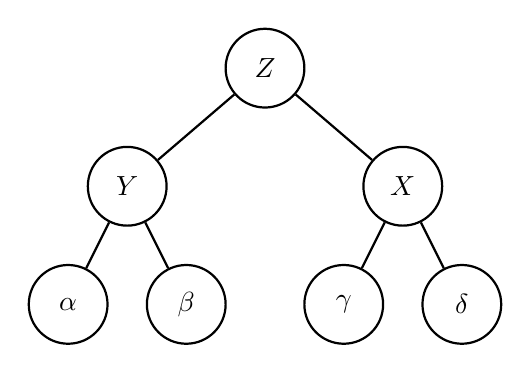
\begin{tikzpicture}[
                    thick,
                    every node/.style = {draw, circle, minimum size=10mm},
                    level 1/.style = {sibling distance=35mm},
                    level 2/.style = {sibling distance=15mm}, 
                    level 3/.style = {sibling distance=15mm}, 
                    level distance = 15mm
                ]
                \node {$Z$}
                    child {node {$Y$}
                        child {node {$\alpha$}}
                        child {node {$\beta$}}
                    }
                    child {node {$X$}
                        child {node {$\gamma$}}
                        child {node {$\delta$}}
                    };
            \end{tikzpicture}
        \end{tabular}
    \end{center}
\end{definition}
\begin{note}
    Аналогично определяется большой левый поворот. 
\end{note}
Нетрудно доказать простой проверкой, что инвариант ДДП сохранится. 

\begin{note}
    Аналогично малому повороту, относительно данного ребра можно сделать только один из больших поворотов.
\end{note}

Рассмотрим теперь новую версию операции $insert(x)$. Заметим, что если мы вставим вершинку так же, как делали и раньше, то инвариант мог сломаться только на пути от новой вершинки до корня. Давайте будем подниматься вверх от только что вставленной вершинки, пересчитывая высоту. Пусть мы находимся в какой-то вершинке $X$ с высотой $h + 3$, у ее левого сына $L$ высота $h + 2$, а у правого $h$ (симметричный случай с правым сыном рассматривается аналогично). Рассмотрим два случая:
\begin{enumerate}
    \item У $L$ высота его левого сына не меньше высоты его правого сына. \\
    Заметим, что тогда обязательно высота левого сына $L$ равна $h+1$, а правого либо $h$, либо $h+1$. Сделаем малый поворот по ребру между $X$ и $L$. Тогда высоты детей сохранятся (высота левого сына $L$ будет $h+1$, левого сына $X$ будет $\in [h, h+1]$, правого сына $X$ будет $h$), тогда высота $X$ будет $\in [h+1, h+2]$, но тогда у $L$ высота будет $\in [h+2, h+3]$. Заметим, что все зависит от высоты левого сына $X$, и в обоих случаях инвариант сохраняется.
    \item У $L$ высота его левого сына меньше высоты его правого сына. \\
    Заметим, что тогда обязательно высота левого сына $L$ равна $h$, а правого $h+1$. Сделаем большой поворот по ребру между $X$ и $L$. Тогда легко однозначно восстановить все новые высоты, у корня будет высота $h+2$, у его детей $h+1$, и легко проверить, что инвариант сохранится.
\end{enumerate}

Остальные операции делаем, как и в обычном ДДП.



\subsection{Корректность}



\begin{proposition}
    Если было дерево высоты $h_{old}$, то после вставки новой вершинки будет выполнено $h_{new} \in [h_{old}, h_{old}+1]$.
\end{proposition}
\begin{proof}
    Докажем по индукции. Пусть у нас было дерево высоты $h$, рассмотрим несколько случаев.
    \begin{enumerate}
        \item Высоты поддеревьев равны $h-1$. \\
        Тогда высота какого-то из поддеревьев, по предположению индукции, стала $\in [h-1, h]$, и высота всего дерева $\in [h, h+1]$, инвариант соблюдается.
        \item Высоты поддеревьев $h-1$ и $h-2$. \\
        Если вставка была в поддерево с меньшей высотой, то, по предположению индукции, новая высота в нем $\in [h-2, h-1]$, инвариант соблюдается. Если же в поддерево с большей высотой, то либо высота не изменилась и все хорошо, либо у дерева высота стала $h+1$, а в поддеревьях высоты равны $h$ и $h-2$. Заметим, что этот случай мы уже разбирали выше при описании операции вставки вершинки, и его мы исправляем просто одним поворотом.
    \end{enumerate}
\end{proof}

\begin{note}
    Аналогично можно доказать, что при обычном удалении $h_{new} \in [h_{old}-1, h_{old}]$, то есть инвариант тоже сохраняется.
\end{note}

Таким образом, все операции, изменяющие дерево, сохраняют инвариант, поэтому теперь все операции, которые работали за $O(h)$ (в том числе $insert(x)$) теперь работают за $O(log_2(n))$.



\section{Красно-черное дерево}



У AVL-Дерева есть некоторые проблемы, например, память, т. к. в каждой вершине надо хранить высоту и постоянно пересчитывать ее, а еще приходится делать $O(log_2(n))$ поворотов за одну операцию. Поэтому стали придумывать другие деревья, и даже, например, в STL C++ используется другое ДДП для std::set, а именно красно-черное. В нем каждая вершинка либо красного, либо черного цвета, а еще листьями всегда являются ``нулевые'' вершинки (или же одна фиктивная вершинка, которая выполняет роль нулевой), причем их цвет всегда черный.

\begin{invariant}
    Корень всегда черный.
\end{invariant}
\begin{invariant}
    Если вершинка красная, то оба ее сына черные.
\end{invariant}
\begin{invariant}
    Для каждой вершинки все простые пути до листьев среди ее потомков содержат одинаковое количество черных вершин.
\end{invariant}

Заметим, что красно-черное дерево может быть не сбалансировано с точки зрения AVL. А еще заметим, что на любом пути от черной вершинки до любого листа не более половины вершин красные. Интуитивно понятно, что дерево без красных вершин как-будто бы очень хорошо сбалансировано, а если есть красные вершинки, то они где-то между черными и не сильно все портят.

\begin{definition}
    $bh(x)$ (черная высота) -- количество черных вершин на простом пути от вершины $x$ до любого листа (без учета цвета $x$).
\end{definition}

\begin{lemma}
    В поддереве черной вершины $x$ есть как минимум $2^{bh(x)} - 1$ черных вершин.
\end{lemma}
\begin{proof}
    Можно легко доказать по индукции.
\end{proof}

\begin{lemma}
    Красное-черное дерево с $n$ вершинами имеет высоту не более, чем $2log_2(n+1)$.
\end{lemma}
\begin{proof}
    Можно доказать через предыдущую лемму.
\end{proof}



\subsection{Операции в красно-черном дереве}



\subsubsection{Операция insert(x)}

Если мы хотим вставить новую вершинку $Z$, то сделаем вставку из обычного ДДП и покрасим новую вершинку в красный цвет. Если предок новой вершинки черный -- то все хорошо, а если красный, то вызовем некоторую функцию $RB\_Insert\_Fixup(x)$, которая все исправит, делая некоторые повороты и перекраски. \pagebreak

Примерный код тупой вставки: \\

\begin{lstlisting}
    void RB_Insert(T, z) {
        y = T.nil
        x = T.root
        while (x != T.nil) {
            y = x
            if (z.key < x.key) {
                x = x.left
            } else {
                x = x.right
            }
        }

        z.p = y
        if (y == T.nil) {
            T.root = z
        } else if (z.key < y.key) {
            y.left = z
        } else {
            y.right = z
        }

        z.left = T.nil
        z.right = T.nil
        z.color = RED
        RB_Insert_Fixup(T, z);
    }
\end{lstlisting}

Где $T.nil$ -- тот самый сжатый нулевой лист, $T$ -- дерево, $z$ -- готовая вершина, которую надо вставить. \\
При такой вставке может нарушиться инвариант $3.1$ (если вставили в пустое дерево) или $3.2$. В первом случае просто заифаем и покрасим вершинку в черный, а для второго разберем функцию $RB\_Insert\_Fixup(x)$. 

Пусть у $x$ родитель $p$ (оба они красного цвета), у $p$ родитель $g$ (он обязательно черный), а $u$ -- второй сын $g$ (брат $p$, или же дядя $x$). \\
Если $u$ красного цвета, то перекрасим $p$ и $u$ в черный, а $g$ в красный. Если нарушился инвариант $3.1$, то тогда $g$ -- корень, и его можно просто покрасить в черный. Если же нарушился инвариант $3.2$, то тогда отец $g$ -- тоже красный, и мы можем запустить эту функцию еще раз рекурсивно выше. Легко доказать, что если так делать, то никогда не нарушится инвариант $3.3$ \\ 
Если $u$ черного цвета или отсутствует, то пусть $x$ и $p$ являются левыми/правыми детьми своих родителей. Тогда просто сделаем малый поворот по ребру между $p$ и $g$ и поменяем их цвета местами. Легко доказать, что и тут сохранятся все инварианты, и более того, на этом выполнение функции заканчивается. \\
Если же $p$ -- левый ребенок, а $x$ -- правый, или наоборот, то сделаем малый поворот по ребру между $x$ и $p$, и перейдем к предыдущему случаю (то есть по сути мы сделаем большой поворот). \\
Таким образом, пока наш дядя красный, мы просто перекрашиваем вершины и поднимаемся наверх, а если он в какой-то момент стал черным (или перестал существовать), то мы сделаем не более двух поворотов. Другими словами, $RB\_Insert\_Fixup(x)$ делает $O(log_2(n))$ перекрашиваний и $O(1)$ поворотов, что является одним из преимуществ красно-черного дерева над AVL-деревом, ведь в каждом повороте мы меняем дерево и что-то переподсчитываем, что работает хоть и за $O(1)$, но за немалую константу.

\begin{note}
    Возможно, что если ввести потенциал как количество красных вершин, то можно доказать, что $RB\_Insert\_Fixup(x)$ работает амортизированно за $O(1)$.
\end{note}

\subsubsection{Операция erase(x)}

Так же, как и в обычном ДДП, если у $x$ есть два ребенка, то поменяем ее местами с другой вершиной так, чтобы у нее остался не более чем один ребенок (меняем местами только значения, не цвета). Если $x$ красного цвета, то проблем нет -- просто удаляем ее и ставим на ее место ребенка, если он есть. Если $x$ черного цвета и у него есть ребенок, то этот ребенок обязательно красный, причем без детей (иначе будет нарушен инвариант $3.3$, мы ведь цвета не меняли). Тогда тоже просто удаляем и ставим на свое место ребенка, перекрасив его в черный цвет. Если же $x$ черного цвета без детей, то, если он корень, то все тривиально, а иначе начинаются проблемы. \\
Для начала удалим вершину $x$, из-за этого найдется такая вершина $X$, что у нее есть такой брат, что их черные глубины отличаются. Если $X$ красного цвета или корень поддерева, то просто перекрасим его в черный. Иначе рассмотрим 4 случая:

\begin{enumerate}
    \item Брат $B$ вершинки $X$ красный. \\
    Сделаем малый поворот по ребру между $P$ (отец $X$, точно черный) и $B$ и поменяем цвета у $P$ и $B$, получим случай $2$.
    \item $B$ черный, дети $X$ черные. \\
    Покрасим $B$ в красный цвет. Если $P$ красный, то покрасим его в черный и завершимся, иначе рекурсивно продолжим от $P$.
    \item $B$ черный, ближний племянник к $X$ красный, а дальний черный (ближний племянник -- левый сын $B$, если $X$ левый сын $P$, и наоборот, дальний племянник -- сын вершины $B$, отличный от ближнего племянника). \\
    Поменяем цвета у красного племянника и $B$, потом сделаем малый поворот по ребру между этим племянником и $B$ и перейдем к другому случаю.
    \item $B$ черный, дальний племянник к $X$ красный. \\
    Поменяем цвета у $P$ и $B$ и сделаем малый поворот по ребру между $P$ и $B$, а еще покрасим дальнего племянника к $X$ в черный цвет.
\end{enumerate}

Таким образом мы умеем делать все операции за $O(log_2(n))$ перекрашиваний и $O(1)$ поворотов, что часто неасимптотически быстрее, чем AVL-дерево. \pagebreak
